\chapter{永磁同步电机矢量控制仿真}
\section{引言}
在掌握永磁同步电机建模以及矢量控制基本原理之后,通过Matlab/Simulink软件搭建永磁同步电机矢量控制系统,进行仿真分析。本章主要介绍永磁同步电机矢量控制的仿真模型,包括永磁同步电机子系统、控制器子系统以及基于反电动势位置估算算法子系统。
\section{Matlab/Simulink软件介绍}
Mathworks公司的Matlab软件无疑是当前应用最为广泛的矩阵计算与数值分析软件,广泛应用于科研教学以及工业研发场合。对于电机控制研究来讲,主要使用Simulink软件,通过在Simulink图形方式搭建系统仿真模型,分析系统动态响应,十分方便。Simulink本身内置许多工具箱库,比如说电力系统库(SimPowersystem)可专门用于电气传动仿真研究。此外,Simulink软件另一个十分有用的模块是S-函数模块,可用于编写自定义功能模块,十分灵活。S-函数采用Matlab代码、C语言或者$C++$实现\cite{matlab}。
\section{永磁同步电机矢量控制系统仿真}
利用Simulink搭建的永磁永磁同步电机矢量控制仿真模型主要包括永磁同步电机子系统和离散控制器子系统。为了简化分析,本仿真模型假设逆变器为理想逆变器,即逆变器输出电压与给定完全一致,这样在仿真模型中就可以省去逆变器模型与控制矢量调制法,直接将控制器输出的电压指令连接到永磁同步电机子系统。
\section{永磁同步电机子系统}
Simulink的工具箱中提供了电机模块可以直接用,但是为了方便研究,根据永磁同步电机数学模型,采用Simulink搭建永磁永磁同步电机子系统。子系统如图\ref{fig:PMSM_subsystem}所示,其包含三相电压、负载输入端口,包含转速、电磁转矩、三相电流和转子位置输出端口。
\begin{figure}[H]
	\centering
	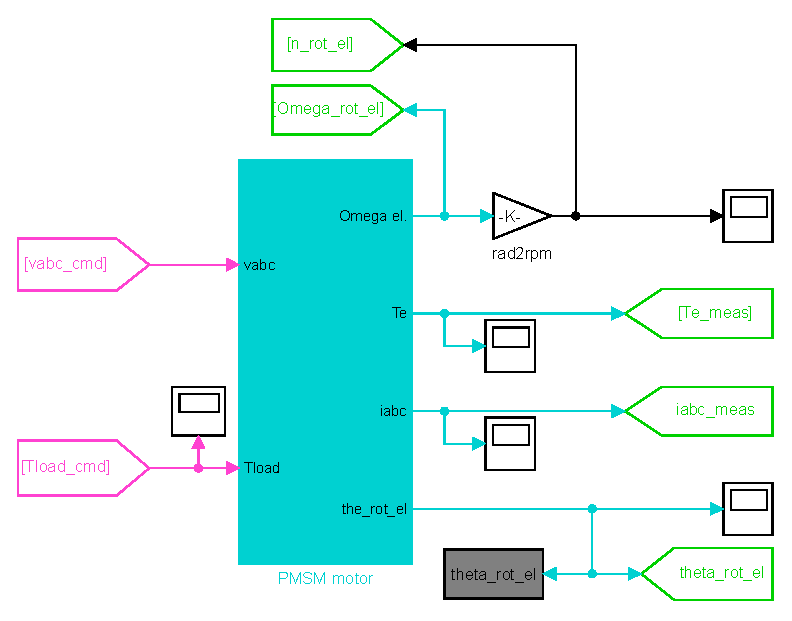
\includegraphics[width=0.7\textwidth]{figs/PMSM_subsystem.eps}
	\caption{永磁同步电机电路模型}
	\label{fig:PMSM_subsystem}
\end{figure}
永磁同步电机Simulink子系统内部主要包括永磁同步电机电路模型和机械模型,其中电路模型如图\ref{fig:PMSM_model}所示,对应dq坐标系中永磁同步电机的电压方程\ref{eq:vdq_final}和磁链方程\ref{eq:fluxdq_final},机械模型如图\ref{fig:PMSM_model_mec}所示,对应运动平衡方程\ref{eq:mechanical}。为了简化分析,其中机械模型忽略了方程\ref{eq:mechanical}中的摩擦转矩项。
\begin{figure}[H]
	\centering
	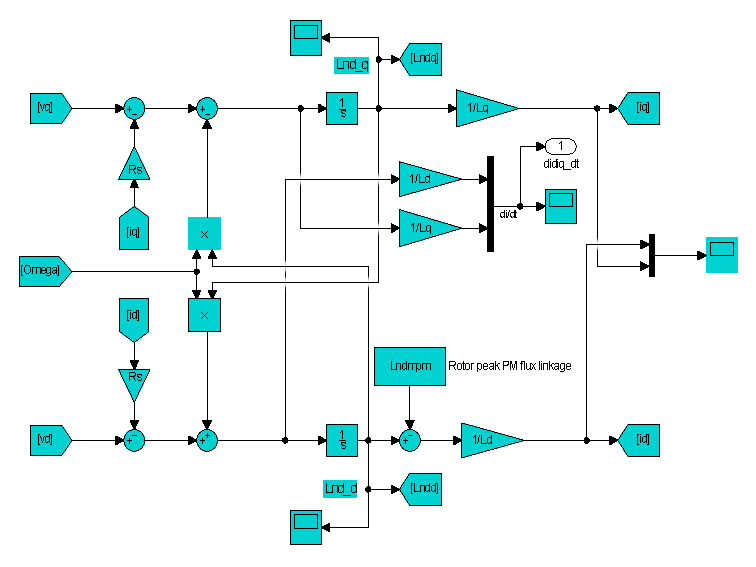
\includegraphics[width=0.7\textwidth]{figs/PMSM_model.eps}
	\caption{永磁同步电机电路模型}
	\label{fig:PMSM_model}
\end{figure}
\begin{figure}[H]
	\centering
	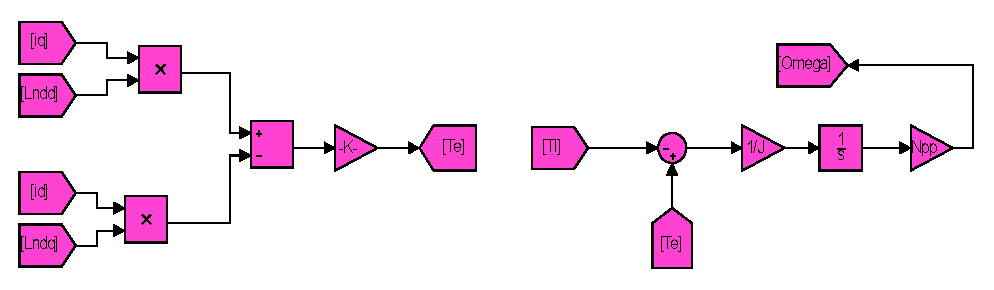
\includegraphics[width=0.7\textwidth]{figs/mechanical.eps}
	\caption{永磁同步电机机械模型}
	\label{fig:PMSM_model_mec}
\end{figure}
\section{矢量控制器子系统}
永磁同步电机矢量控制器子系统如图\ref{fig:controller_subsystem}所示,实际电机控制器一般用DSP芯片,主程序放在PWM中断中,每一个PWM周期执行一次,因此本仿真系统控制器子系统采用触发的方式运行,触发形式为上升沿触发,触发频率为5kHz。这样做相当于采用DSP控制,开关频率为5k。可以看到该矢量控制子系统输入端口为电流采样与电机转子位置,输出为电机电压给定。
\begin{figure}[H]
	\centering
	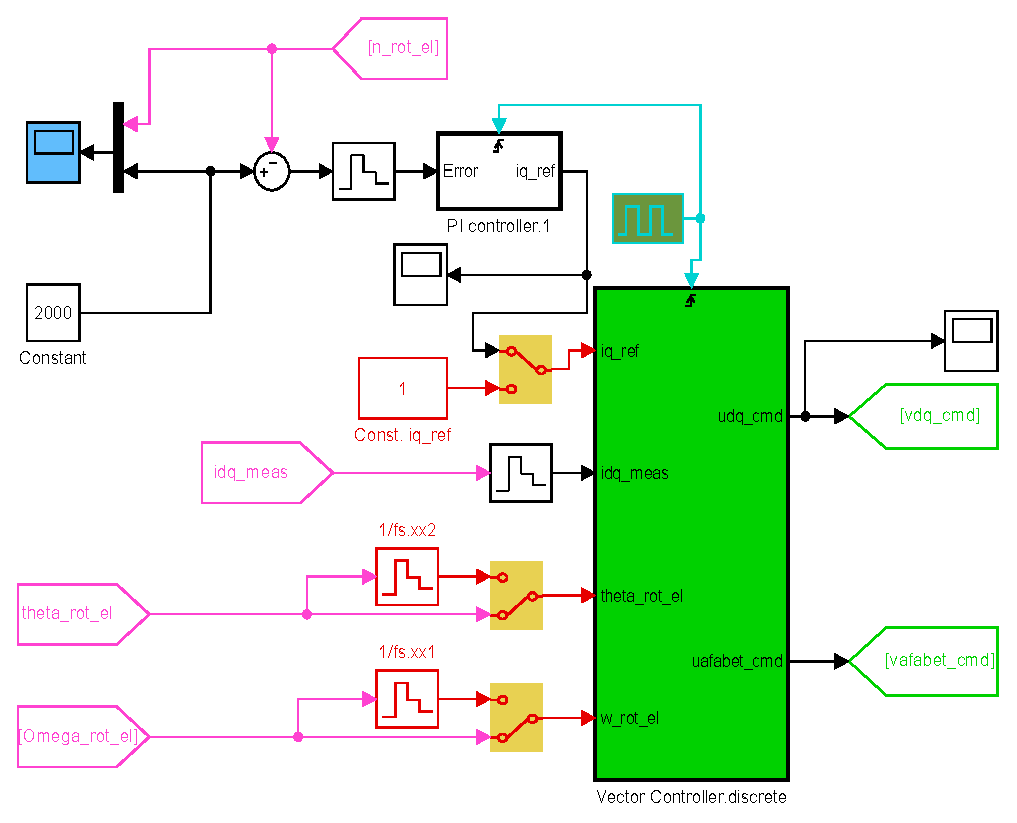
\includegraphics[width=0.7\textwidth]{figs/controller_subsystem.eps}
	\caption{永磁同步电机矢量控制器子系统}
	\label{fig:controller_subsystem}
\end{figure}
永磁同步电机矢量控制子系统内部主要包括两个电流内环以及反电动势解耦模块。如图\ref{fig:controller_inside}所示,根据该图可以看到矢量控制器中$i_{q}$给定来自转速外环$PI$控制器的输出,$i_{d}$给定为0。这与矢量控制结构图\ref{fig:focStructure}对应。
\begin{figure}[H]
	\centering
	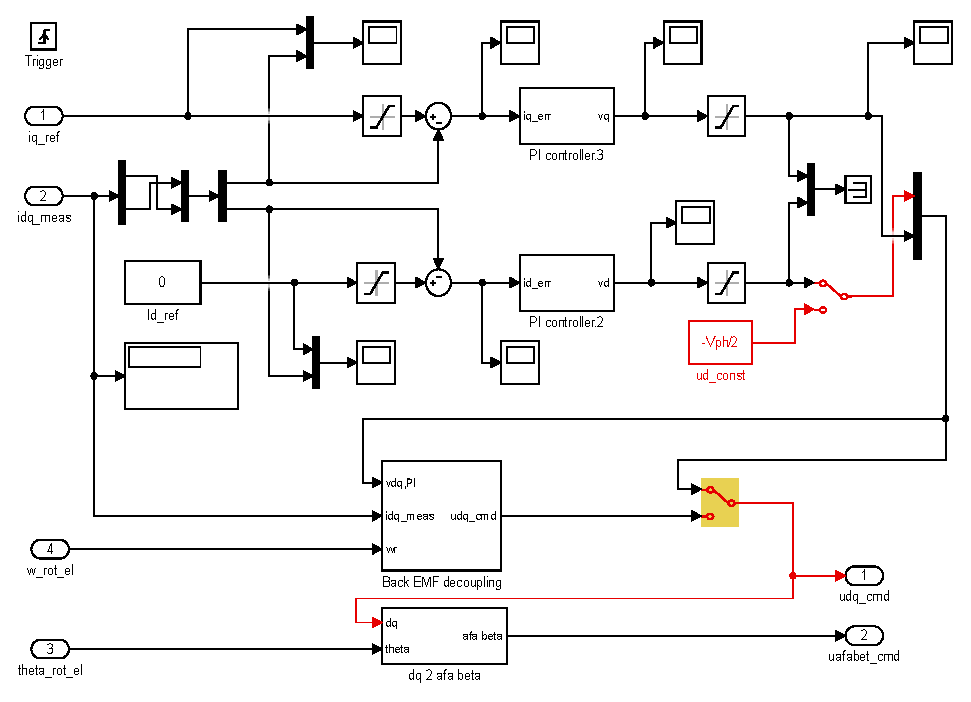
\includegraphics[width=0.7\textwidth]{figs/controller_inside.eps}
	\caption{永磁同步电机矢量控制器子系统内部}
	\label{fig:controller_inside}
\end{figure}
由于dq坐标系中,电机电压方程存在交叉耦合,采用反电动势解耦可简化dq轴电流控制。图\ref{fig:EMF_decouple}所示为反电动势解耦模块,其输入为电流环PI控制器输出的电压指令、电机转速和dq轴电流,通过dq轴电流和电机转速计算出耦合项并进行补偿。
\begin{figure}[H]
	\centering
	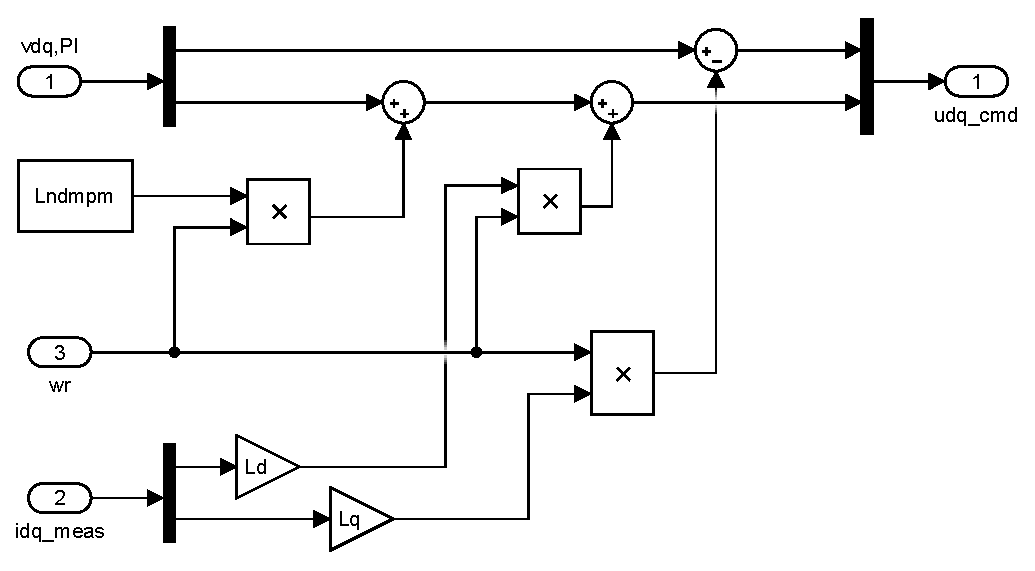
\includegraphics[width=0.7\textwidth]{figs/EMF_decouple.eps}
	\caption{反电动势解耦子系统}
	\label{fig:EMF_decouple}
\end{figure}
由于矢量控制器在采用触发模式执行,控制器中的PI模块需要用离散的积分,图\ref{fig:qpi}为q轴电流环PI控制器子系统,d轴PI控制器与此类似。
\begin{figure}[H]
	\centering
	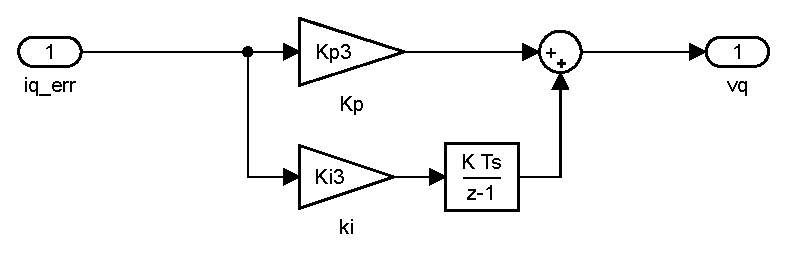
\includegraphics[width=0.7\textwidth]{figs/qpi.eps}
	\caption{离散PI控制器}
	\label{fig:qpi}
\end{figure}
图\ref{fig:anti_windup_pi}为转速闭环抗饱和PI控制器,根据第三章的分析,抗饱和PI控制器在输出未饱和时与传统PI控制器一样,但输出饱和时,其能更快地是控制器退出饱和,能够减少系统超调。
\begin{figure}[H]
	\centering
	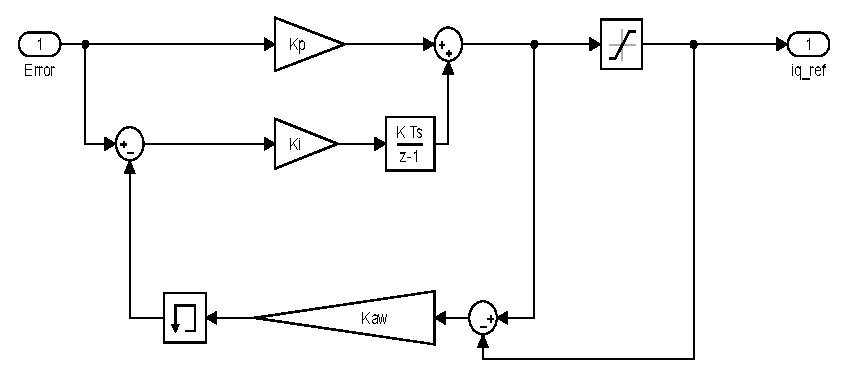
\includegraphics[width=0.7\textwidth]{figs/anti_windup_pi_speed.eps}
	\caption{离散抗饱和PI控制器}
	\label{fig:anti_windup_pi}
\end{figure}
\section{仿真调试}
永磁同步电机矢量控制系统中的三个PI控制器参数调试时矢量控制的重点。实际调试时,先将速度外环断开,调节电流环PI控制参数,一般在电机静止的情况下调节d轴控制器,q轴电流控制器参数与d轴参数相同。调节好电流环之后,调节包含电流内环的转速环。

本仿真系统采用的永磁同步电机参数为:额定电流6.8A,d轴电感1.7mH,q轴电感1.7mH,绕组电阻$R=0.353\Omega$额定转矩3.18Nm,转动惯量$J=2.1*10^{-4}$,额定频率250Hz,5对极,仿真所用开关频率5KHz。电流环控制器参数为:$K_{p}=5.37$,$K_{i}=1106$,转速环控制器参数为:$K_{p}=0.1$,$K_{i}=10$,$K_{aw}=12$。

\subsection{仿真结果分析}
电机转速给定为1000rpm,d轴电流参考值为0,负载转矩初始值为0,在0.1s时阶跃值2.54Nm。仿真过程中对电机转速、电磁转矩、相电流、励磁电流、基于反电动势位置估算值波形进行观察分析。

图\ref{fig:speed}为电机转速响应波形,空载时,电机转速能够很快跟上给定转速。在0.1s加80\%额定负载时,转速下降约90RPM,在0.02s之内上升至稳定值。
\begin{figure}[H]
	\centering
	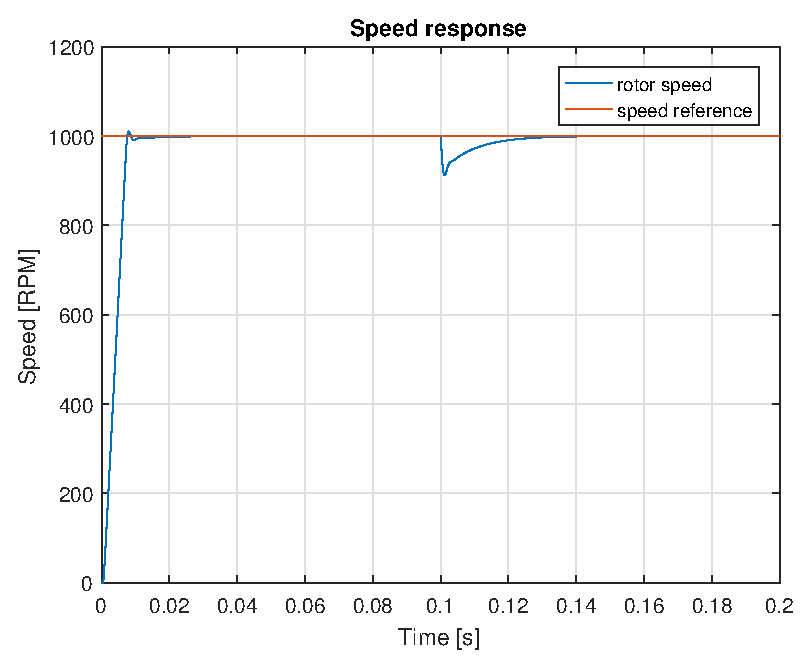
\includegraphics[width=0.7\textwidth]{figs/speed.eps}
	\caption{转速}
	\label{fig:speed}
\end{figure}
图\ref{fig:torque}为电机输出电磁转矩,启动阶段,可以看到电机输出额定电磁转矩,此时电机以最大加速度加速,稳定时输出转矩等于负载转矩。
\begin{figure}[H]
	\centering
	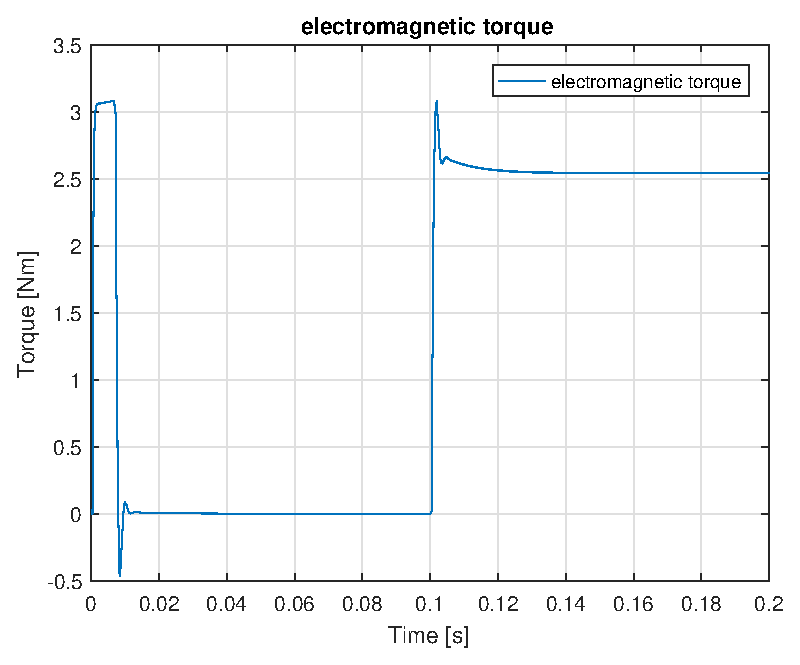
\includegraphics[width=0.7\textwidth]{figs/torque.eps}
	\caption{电磁转矩}
	\label{fig:torque}
\end{figure}
图\ref{fig:iabc}为定子三相电流波形,可以看电机加速阶段,电流很大。空载时,永磁同步电机三相电流几乎为零,0.1秒加上负载转矩时,电流变大,提供q负载转矩。
\begin{figure}[H]
	\centering
	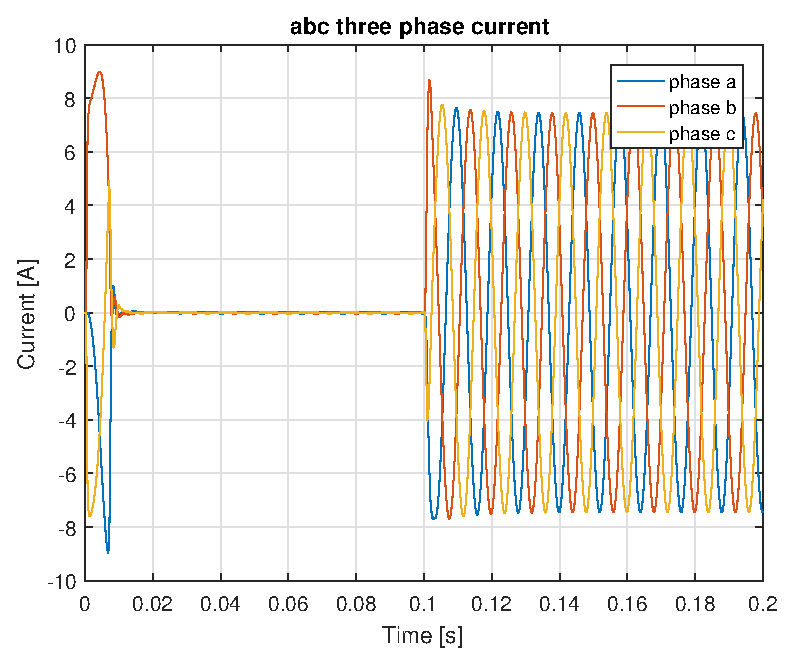
\includegraphics[width=0.7\textwidth]{figs/iabc.eps}
	\caption{abc定子三相电流}
	\label{fig:iabc}
\end{figure}
图\ref{fig:id}为电机d轴电流波形,可以看到在启动加速阶段与突加负载时,d轴电流均存在较小脉冲(最大0.3A),这是由于耦合项造成的。仿真时使用了反电动势解耦,但是在瞬态过程中,并没有完美解耦。图\ref{fig:id_without_decouple}为不使用解耦时,其他条件完全一样的d轴电流响应,可以看到不使用解耦时,d轴电流冲击最大幅值越为1.2A是使用解耦时响应冲击电流的4倍,由此反电动势解耦可以降低瞬态过程中的电流冲击,使系统响应更加平滑。
\begin{figure}[H]
	\centering
	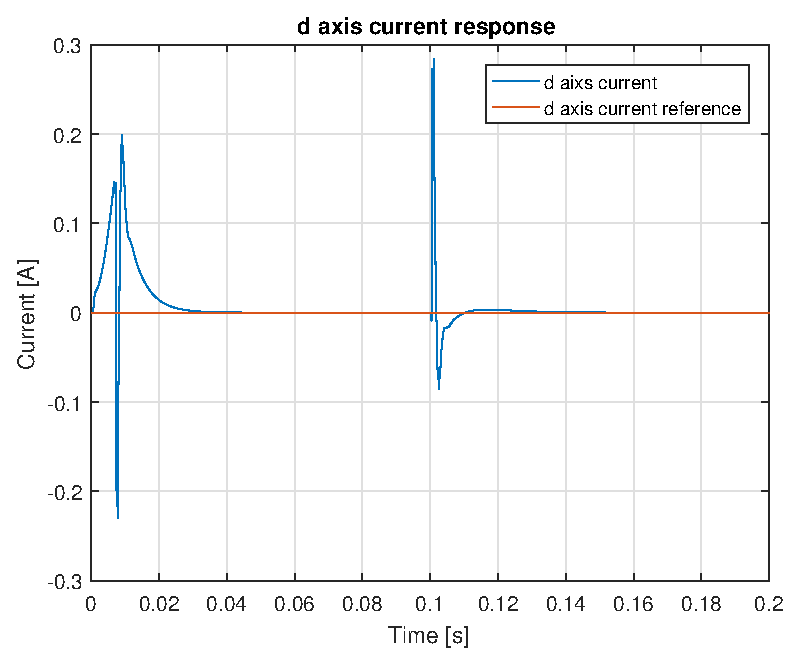
\includegraphics[width=0.7\textwidth]{figs/id.eps}
	\caption{d轴电流}
	\label{fig:id}
\end{figure}
\begin{figure}[H]
	\centering
	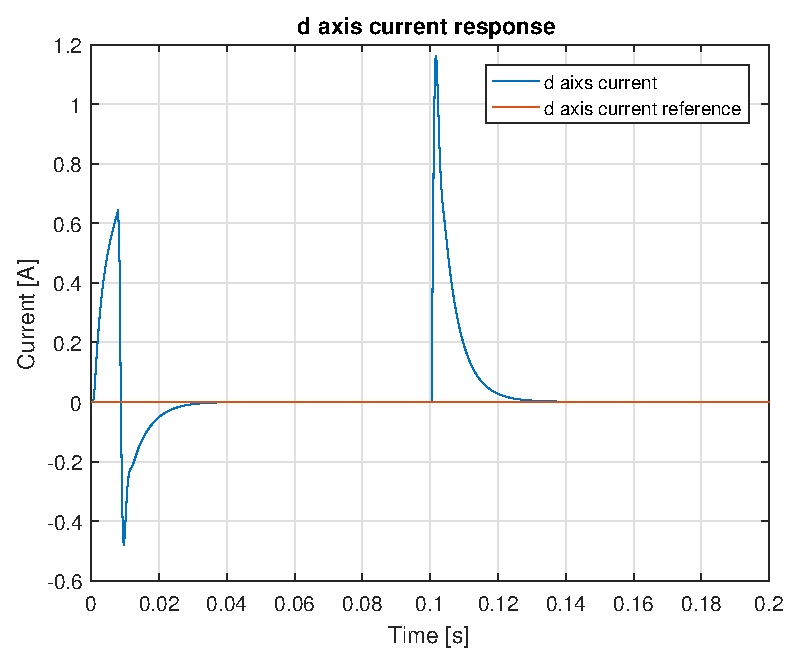
\includegraphics[width=0.7\textwidth]{figs/id_without_decouple.eps}
	\caption{不使用反电动势解耦时d轴电流响应}
	\label{fig:id_without_decouple}
\end{figure}
图\ref{fig:iq}为q轴电流响应,可以看到q轴在加速阶段电流接近最大电流,此时电机以最大加速加速,在空载匀速阶段,由于仿真忽略了磨擦转矩,因此电流为0,在0.1s加负载时,q轴电流迅速上升,来提供转矩最终使得转速恒定。最终稳定时,理论电流值$i_{q}=\frac{T_{l}}{\frac{3}{2}P\lambda_{mpm}}=7.44A$,该图与理论符合。
\begin{figure}[H]
	\centering
	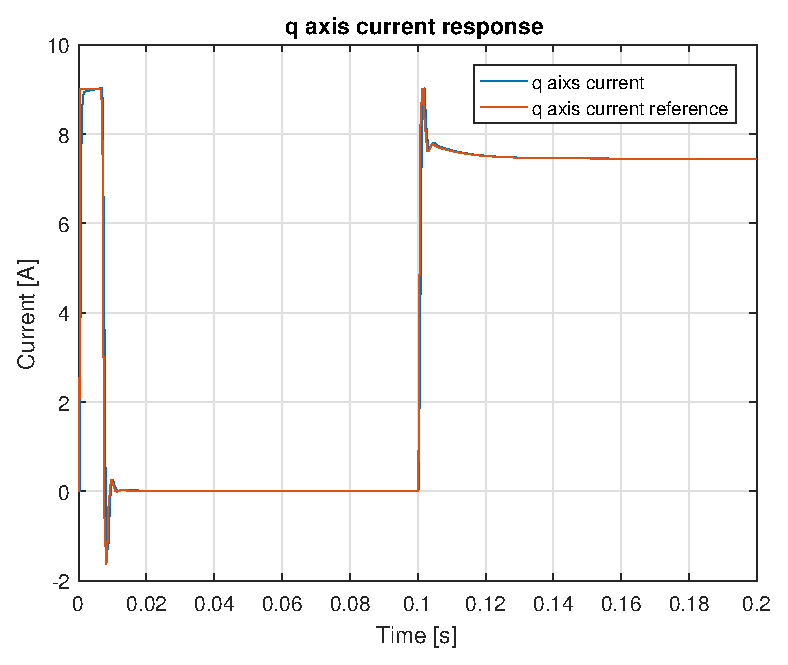
\includegraphics[width=0.7\textwidth]{figs/iq.eps}
	\caption{q轴电流}
	\label{fig:iq}
\end{figure}
图\ref{fig:flux}和\ref{fig:position_estimation}为反电动势位置估算方法中用于计算转子位置的$\alpha\beta$磁链轨迹和估算的转子位置。开始由于电机转速较低,反电动势数值太小,该方法不准确,此时磁链轨迹不为圆心在坐标原点的圆,估算的转子位置与实际转子位置偏差较大,后来磁链轨迹圆心基本稳定与坐标原点,此时估算的转子位置与实际转子位置基本吻合。
\begin{figure}[H]
	\centering
	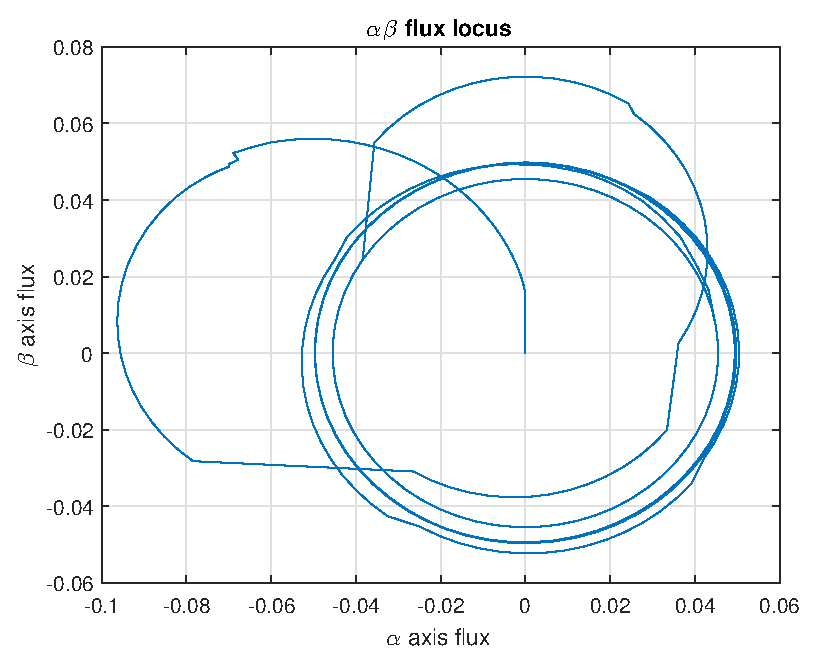
\includegraphics[width=0.7\textwidth]{figs/flux.eps}
	\caption{$\alpha\beta$ 磁链轨迹}
	\label{fig:flux}
\end{figure}
\begin{figure}[H]
	\centering
	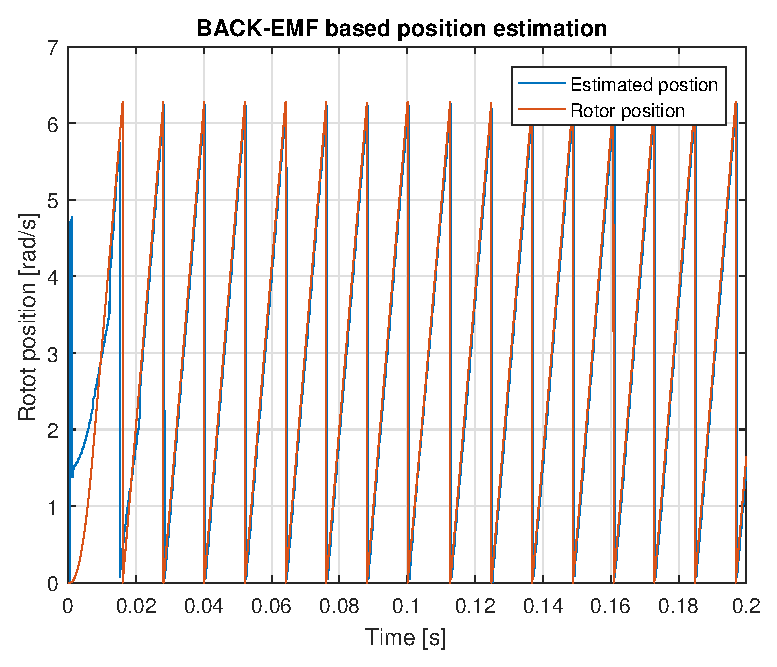
\includegraphics[width=0.7\textwidth]{figs/position_estimation.eps}
	\caption{位置估算}
	\label{fig:position_estimation}
\end{figure}
\section{本章小结}
本章根据永磁同步电机dq数学模型详细描述了永磁同步电机矢量原理。在理解原理基础之上,建立了基于Simulink的永磁同步电机矢量控制系统仿真模型,基于反电动势位置估算方法模型,进行仿真并对仿真结果进行详细的分析。